\documentclass[12pt,a4paper]{article}
\usepackage[T2A]{fontenc}
\usepackage[utf8]{inputenc}
\usepackage[ukrainian]{babel}
\usepackage[left=2.5cm,right=2cm,top=2cm,bottom=2.5cm]{geometry}
\usepackage{graphicx}
\usepackage{float}
\usepackage{booktabs}
\usepackage{array}
\usepackage{amsmath}
\usepackage[labelsep=colon]{caption}
\usepackage{enumitem}
\usepackage{fancyvrb}
\usepackage{indentfirst}
\usepackage{tikz}
\usetikzlibrary{positioning,arrows.meta,shapes.geometric}

\graphicspath{{figures/}}
\fvset{fontsize=\small,frame=single,framesep=2mm}
\setlist[enumerate]{leftmargin=*}
\setlength{\parskip}{0.3em}
\setlength{\emergencystretch}{3em}

% Титульна сторінка: #1 — номер лабораторної роботи
\newcommand{\labtitlepage}[1]{%
\begin{titlepage}
\begin{center}
\large
Міністерство освіти і науки України\\
Національний університет ``Львівська політехніка''\\
Кафедра прикладної математики
\vspace*{\fill}

{\LARGE Звіт}\\[0.5em]
{\Large про виконання лабораторної роботи №#1}\\[0.5em]
{\Large з курсу «Основи інженерії даних»}
\vspace*{\fill}
\end{center}
\begin{flushright}
\begin{minipage}{0.4\textwidth}
\large
Виконала:\\
студентка групи ПМІД-11\\
Мазур Д. М.\\[1.5em]
Перевірив:\\
Алєксєєв В. І.
\end{minipage}
\end{flushright}
\vspace*{\fill}
\begin{center}
\large Львів — 2026
\end{center}
\end{titlepage}
\setcounter{page}{2}}

\newcommand{\rsec}[1]{\par\medskip\noindent\textbf{#1}\ }

\tikzset{
  tbl/.style={draw, rounded corners=2pt, align=left, font=\scriptsize\ttfamily, inner sep=3pt},
  fact/.style={tbl, very thick},
  rel/.style={-{Stealth[length=2mm]}, thin}
}
\begin{document}
\labtitlepage{2}

\rsec{Тема:} Моделювання даних та проектування схем сховища даних: схеми «зірка» та «сніжинка».

\rsec{Мета роботи:} Зрозуміти компроміси між різними парадигмами моделювання даних та те, як проектування схем впливає на продуктивність запитів. Ознайомитися з нормалізацією та денормалізацією, а також логічною структурою схем «зірка» та «сніжинка».

\rsec{Постановка задачі:} Розробити та впровадити нову схему для команди бізнес-аналітики, якій потрібно виконувати швидкі спеціальні (ad-hoc) запити до даних про продажі.

\rsec{Завдання до роботи:}
\begin{enumerate}
  \item Створити схему «зірка» та схему «сніжинка».
  \item Завантажити дані в обидві схеми.
  \item Виконати аналітичні запити для порівняння продуктивності.
\end{enumerate}

\rsec{Хід виконання роботи:}
\begin{enumerate}
  \item \textbf{Вхідні дані та інструменти.} Джерелом даних є CSV-файл із 1\,000\,000 транзакцій, отриманий у лабораторній роботі №1 (поля \texttt{transaction\_id}, \texttt{user\_id}, \texttt{amount}, \texttt{category}, \texttt{status}, \texttt{timestamp}). Як СУБД використано SQLite, а завантаження виконано за допомогою pandas. Код розміщено у \texttt{lab2\_db/scripts/}: \texttt{build\_and\_load.py} будує та заповнює схеми, \texttt{benchmark\_queries.py} виконує порівняння.

  \item \textbf{Проектування схем.} В обох схемах таблиця фактів однакова: одна транзакція — один рядок. Вона містить міру \texttt{amount}, зовнішні ключі вимірів та час транзакції. Зерно (grain) виміру дат обрано рівним одній годині, тому вимір містить 278 рядків замість 1\,000\,000 унікальних секунд. Схеми відрізняються лише організацією вимірів:
  \begin{itemize}
    \item \textbf{«Зірка»} (рис.~\ref{fig:star}): кожен вимір є однією денормалізованою таблицею. Ієрархії зберігаються всередині виміру: група категорії в \texttt{star\_dim\_category}, рік, місяць, день і година в \texttt{star\_dim\_date}.
    \item \textbf{«Сніжинка»} (рис.~\ref{fig:snow}): ієрархії вимірів нормалізовано в окремі таблиці: категорія \(\rightarrow\) група категорій, дата \(\rightarrow\) місяць \(\rightarrow\) рік.
  \end{itemize}

\begin{figure}[H]
\centering
\begin{tikzpicture}[node distance=6mm and 14mm]
\node[fact] (f) {\textbf{star\_fact\_transactions}\\transaction\_id (PK)\\user\_id\\category\_id (FK)\\status\_id (FK)\\date\_id (FK)\\transaction\_ts\\amount};
\node[tbl, left=of f, yshift=10mm] (c) {\textbf{star\_dim\_category}\\category\_id (PK)\\category\_name\\category\_group};
\node[tbl, left=of f, yshift=-12mm] (s) {\textbf{star\_dim\_status}\\status\_id (PK)\\status\_name};
\node[tbl, right=of f] (d) {\textbf{star\_dim\_date}\\date\_id (PK)\\date\_hour\\year, month\\day, hour};
\draw[rel] (f) -- (c); \draw[rel] (f) -- (s); \draw[rel] (f) -- (d);
\end{tikzpicture}
\caption{Схема «зірка»: факт оточений денормалізованими вимірами}
\label{fig:star}
\end{figure}

\begin{figure}[H]
\centering
\begin{tikzpicture}[node distance=5mm and 9mm]
\node[fact] (f) {\textbf{snow\_fact\_transactions}\\transaction\_id (PK)\\user\_id\\category\_id (FK)\\status\_id (FK)\\date\_id (FK)\\transaction\_ts\\amount};
\node[tbl, left=of f, yshift=12mm] (c) {\textbf{snow\_dim\_category}\\category\_id (PK)\\category\_name\\group\_id (FK)};
\node[tbl, left=of c] (g) {\textbf{snow\_dim\_category\_group}\\group\_id (PK)\\group\_name};
\node[tbl, left=of f, yshift=-14mm] (s) {\textbf{snow\_dim\_status}\\status\_id (PK)\\status\_name};
\node[tbl, right=of f, yshift=12mm] (d) {\textbf{snow\_dim\_date}\\date\_id (PK)\\date\_hour\\day, hour\\month\_id (FK)};
\node[tbl, below=of d] (m) {\textbf{snow\_dim\_month}\\month\_id (PK)\\month\_val\\year\_id (FK)};
\node[tbl, below=of m] (y) {\textbf{snow\_dim\_year}\\year\_id (PK)\\year\_val};
\draw[rel] (f) -- (c); \draw[rel] (c) -- (g); \draw[rel] (f) -- (s);
\draw[rel] (f) -- (d); \draw[rel] (d) -- (m); \draw[rel] (m) -- (y);
\end{tikzpicture}
\caption{Схема «сніжинка»: ієрархії вимірів винесено в окремі таблиці}
\label{fig:snow}
\end{figure}

  \item \textbf{Завантаження даних.} Значення вимірів і сурогатні ключі формуються в pandas один раз і використовуються для обох схем. Тому обидві схеми містять ідентичні дані, і порівняння є чесним. Таблиця фактів формується злиттям (\texttt{merge}) сирих даних з вимірами. Перевірка \texttt{assert len(fact) == len(df)} гарантує, що жоден рядок не втрачено під час зіставлення. Кількість рядків у таблицях наведено в табл.~\ref{tab:rows}. Розмір бази після \texttt{VACUUM} становить 152~MB: по 56~MB на кожну таблицю фактів і по 20~MB на індекси їхніх первинних ключів. Розмір усіх вимірів разом менший за 0.1~MB.

\begin{table}[H]
\centering
\caption{Кількість рядків у таблицях}
\label{tab:rows}
\begin{tabular}{lr@{\hspace{2.5em}}lr}
\toprule
«Зірка» & Рядків & «Сніжинка» & Рядків \\
\midrule
star\_fact\_transactions & 1\,000\,000 & snow\_fact\_transactions & 1\,000\,000 \\
star\_dim\_category & 5 & snow\_dim\_category & 5 \\
 & & snow\_dim\_category\_group & 2 \\
star\_dim\_status & 4 & snow\_dim\_status & 4 \\
star\_dim\_date & 278 & snow\_dim\_date & 278 \\
 & & snow\_dim\_month / snow\_dim\_year & 1 / 1 \\
\bottomrule
\end{tabular}
\end{table}

  \item \textbf{Аналітичні запити.} Для кожної схеми написано три запити, які повертають \emph{однаковий} бізнес-результат. Відрізняється лише кількість з'єднань (JOIN):
  \begin{itemize}
    \item \emph{Q1:} кількість і сума транзакцій за категорією та статусом (по 2 JOIN в обох схемах);
    \item \emph{Q2:} сума за групою категорій і роком (2 JOIN у «зірці», 5 JOIN у «сніжинці»);
    \item \emph{Q3:} поденний дохід від транзакцій COMPLETED за групою категорій (3 JOIN проти 6 JOIN).
  \end{itemize}
  Приклад запиту Q2 для «сніжинки»:
\begin{Verbatim}
SELECT cg.group_name, y.year_val AS year, SUM(f.amount) AS total_amount
FROM snow_fact_transactions f
JOIN snow_dim_category c        ON f.category_id = c.category_id
JOIN snow_dim_category_group cg ON c.group_id = cg.group_id
JOIN snow_dim_date d            ON f.date_id = d.date_id
JOIN snow_dim_month m           ON d.month_id = m.month_id
JOIN snow_dim_year y            ON m.year_id = y.year_id
GROUP BY cg.group_name, y.year_val;
\end{Verbatim}
  У «зірці» той самий результат дає запит лише з двома з'єднаннями, бо \texttt{category\_group} і \texttt{year} уже лежать у вимірах.

  \item \textbf{Методика вимірювання.} Кожен запит виконується один раз для прогріву (перший запуск читає сторінки з диска в кеш). Потім виконуються 5 вимірюваних запусків і береться медіана. Після вимірювань програма перевіряє через \texttt{pd.testing.assert\_frame\_equal}, що результати «зірки» і «сніжинки» збігаються.

  \item \textbf{Результати.} Результати наведено в табл.~\ref{tab:bench} та на рис.~\ref{fig:bench}. Для всіх трьох запитів результати схем збіглися.

\begin{table}[H]
\centering
\caption{Час виконання запитів (медіана 5 запусків)}
\label{tab:bench}
\begin{tabular}{lccrrr}
\toprule
Запит & JOIN (зірка) & JOIN (сніжинка) & Зірка, мс & Сніжинка, мс & Сніжинка / Зірка \\
\midrule
Q1 & 2 & 2 & 452.4 & 462.0 & 1.02x \\
Q2 & 2 & 5 & 299.2 & 340.7 & 1.14x \\
Q3 & 3 & 6 & 113.9 & 123.5 & 1.08x \\
\bottomrule
\end{tabular}
\end{table}

\begin{figure}[H]
\centering
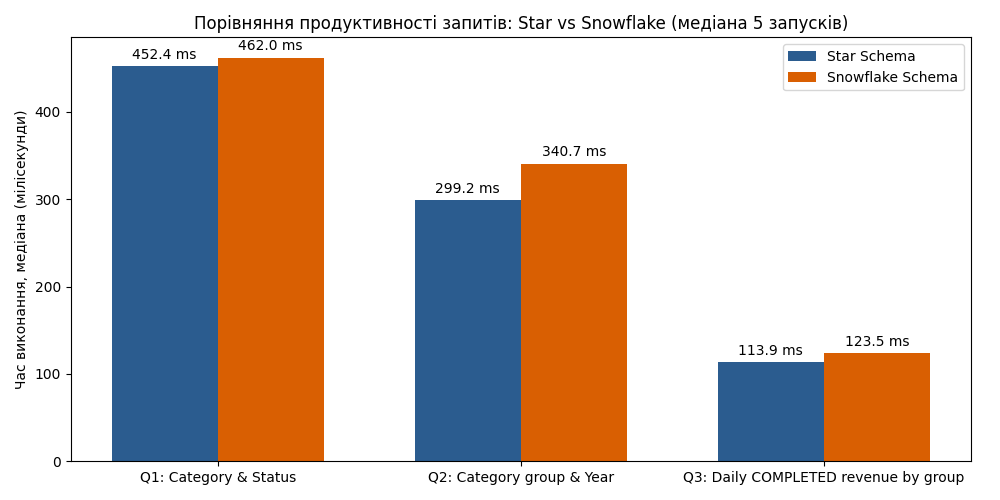
\includegraphics[width=0.72\textwidth]{lab2_benchmark.png}
\caption{Порівняння продуктивності запитів: Star vs Snowflake}
\label{fig:bench}
\end{figure}
\end{enumerate}

\rsec{Висновки:} У ході виконання лабораторної роботи №2 спроектовано та заповнено схеми «зірка» і «сніжинка» для 1\,000\,000 транзакцій у SQLite та порівняно їхню продуктивність на трьох еквівалентних запитах. Коли кількість з'єднань однакова (Q1), час практично не відрізняється (1.02x). Коли запит звертається до рівнів ієрархії (група категорій, рік), «сніжинка» потребує додаткових JOIN і виявляється на 8--14\% повільнішою. SQLite виконує з'єднання вкладеними циклами з пошуком за первинним ключем, тому кожен додатковий вимір означає ще один пошук у B-дереві для кожного з мільйона рядків фактів. Різниця відносно невелика, бо виміри дуже малі й повністю поміщаються в кеш. На реальних сховищах з великими вимірами розрив зростає. Отже, для команди бізнес-аналітики з ad-hoc запитами доцільна схема «зірка»: запити простіші й швидші. «Сніжинка» економить місце й спрощує підтримку цілісності ієрархій, але для невеликих вимірів цей виграш несуттєвий: усі виміри тут займають менше 0.1~MB проти 56~MB таблиці фактів.

\end{document}
